\chapter{Wykład 8. Zarządzanie zakresem projektu i produktu w projekcie informatycznym}

\section{Wymagania}
% strona 16

\begin{table}[htb]
\centering
\begin{tabular}{r|c c c|p{10.5cm}} 
Lp. & TC1 & TC2 & TC3 & Wymaganie \\
\hline
1 & + &  &  & Użytkownik może utworzyć konto \\
2 & + & + & + & Użytkownik może się zalogować \\
3 &  & + &  & PM może tworzyć projekty \\
4 &  & + &  & PM może otwierać procesy \\
5 &  &  &  & PM może zamykać procesy \\
6 &  &  & + & Użytkownik może zamykać zadania \\
7 &  & + &  & PM może dodawać/usuwać/modyfikować nowe zadania \\
8 &  & + &  & PM może przypisywać zadania do użytkowników \\
9 & + &  &  & Administrator oraz PM mogą nadawać role \\
10 & + &  &  & Administrator może weryfikować nowych użytkowników \\
11 & + &  &  & Administrator może przeglądać listę oczekujących \\
12 &  & + & + & Użytkownik oraz PM może dodać/edytować dokument \\
13 &  &  & + & PM może usuwać dokument \\
14 & + & + &  & System umożliwia ograniczenie dostępu do zasobów \\
15 &  & + &  & System tworzy domyślne zadania dla każdego procesu \\
\end{tabular}
\caption{\textbf{Macierz zależności wymagań}}
\label{tab:macierzWymagan}
\end{table}


\textbf{TC 1}
\begin{enumerate}
\item Nowy pracownik zakłada konto
\item Administrator przegląda listę użytkowników i znajduje to konto
\item Administrator weryfikuje je
\item Administrator nadaje mu odpowiednią rolę (np programista)
\item Nowy pracownik może się zalogować
\item Nowy pracownik nie ma dostępu do kluczowych dokumentów (dopóki nie zostanie mu przydzielony odpowiedni dostęp)
\end{enumerate}


\textbf{TC 2}
\begin{enumerate}
\item PM loguje się do systemu
\item PM tworzy nowy projekt
\item System automatycznie generuje podstawowe procesy i szablony dokumentów
\item PM otwiera proces otwarcia
\item PM edytuje dokument otwarcia (uzupełnia wygenerowany szablon)
\item PM modyfikuje informacje dotyczące analizy wymagań (określa deadline)
\item PM przyporządkowuje dwóch analityków do edycji analizy wymagań
\item PM ukrywa dostęp do dokumentu analizy wymagań przed innymi użytkownikami
\end{enumerate}


\textbf{TC 3}
\begin{enumerate}
\item Użytkownik loguje się do systemu
\item Użytkownik oznacza swoje ostatnie zadanie jako wykonane
\item Użytkownik przypadkiem wrzuca list miłosny do repozytorium
\item PM kasuje zbędny dokument
\item PM zamyka proces realizacji
\end{enumerate}

\clearpage

% ===========================================================================

\section{Mapa umysłu dla zakresu projektu}
% strona 22

\begin{figure}[!h]
\centering
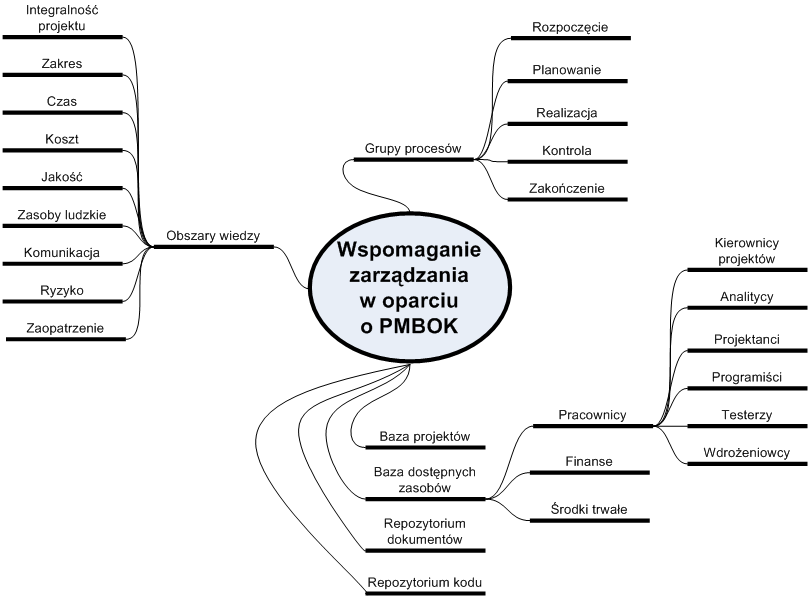
\includegraphics[width=\textwidth]{zakresProjektu.png}
\caption{Zakres projektu}
\label{fig:zakresProjektu}
\end{figure}



